\documentclass{article}
\usepackage{graphicx}
\usepackage{subcaption}

\begin{document}

\begin{figure}[ht]
\centering
\begin{subfigure}[b]{0.33\textwidth}
  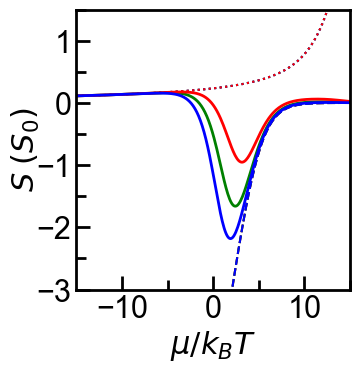
\includegraphics[width=\textwidth]{../Seebeck.png}
\end{subfigure}
\begin{subfigure}[b]{0.33\textwidth}
  \includegraphics[width=\textwidth]{../Conductivity.png}
\end{subfigure}
\begin{subfigure}[b]{0.33\textwidth}
  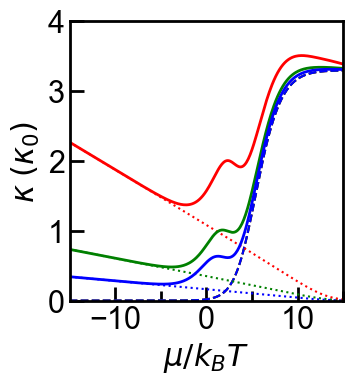
\includegraphics[width=\textwidth]{../Thermal.png}
\end{subfigure}
\begin{subfigure}[b]{0.33\textwidth}
  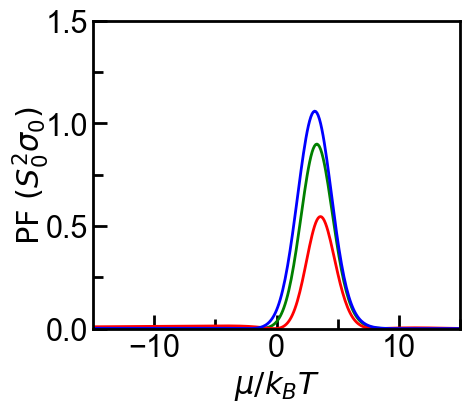
\includegraphics[width=\textwidth]{../PF.png}
\end{subfigure}
\begin{subfigure}[b]{0.33\textwidth}
  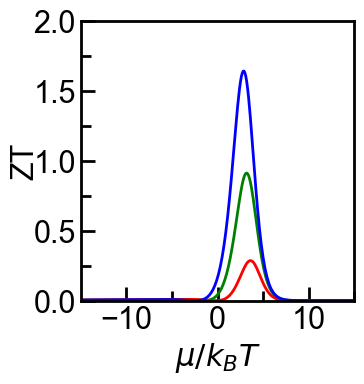
\includegraphics[width=\textwidth]{../ZT.png}
\end{subfigure}
\begin{subfigure}[b]{0.33\textwidth}
    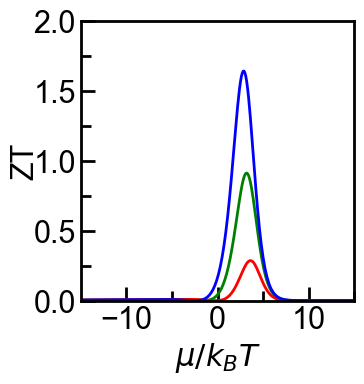
\includegraphics[width=\textwidth]{../ZT.png}
  \end{subfigure}

\caption{Thermoelectric properties of TiS. (a) Seebeck, (b) Conductivity, (c) Thermal, (d)PF, and (e) ZT}
\label{fig:six_images}
\end{figure}

\end{document}
